\documentclass[tikz, border=1mm]{standalone}
\usepackage{structmech}
\usetikzlibrary{calc}

\begin{document}
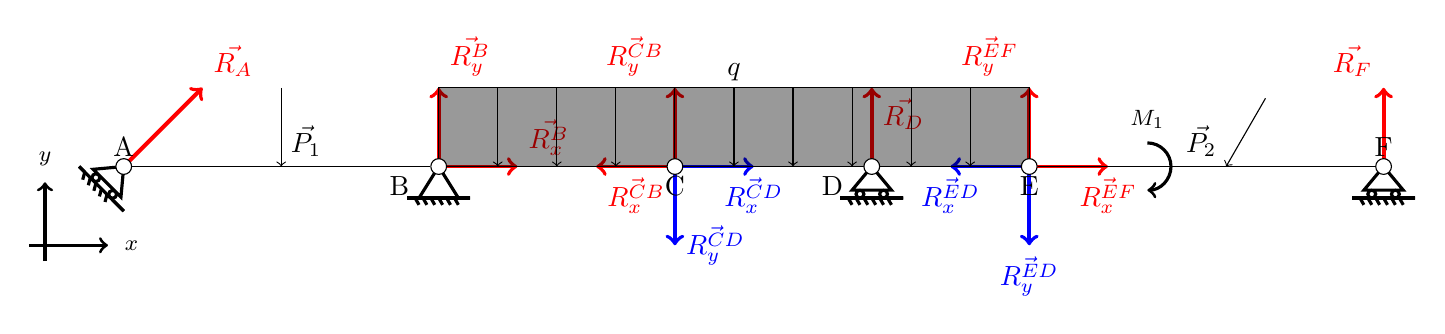
\begin{tikzpicture}
    \CoorOrigin{-1, -1}

    \coordinate (rA) at (0, 0);
    \coordinate (rP1) at (2, 0);
    \coordinate (rB) at (4, 0);
    \coordinate (rC) at (7, 0);
    \coordinate (rD) at (9.5, 0);
    \coordinate (rE) at (11.5, 0);
    \coordinate (rP2) at (14, 0);
    \coordinate (rF) at (16, 0);

    \draw[->] ($(rP1) + (0.0, 1.0)$)--(rP1) node [above right]{$\vec{P_1}$};

    % force P2 applied between E and F with angle 60
    \draw[->] ($(rP2) + ({1.0 * cos(60)}, {1.0 * sin(60)})$)--(rP2) node [above left]{$\vec{P_2}$};

    % display forces Ra, Rby, Rcx, Rcy, Rd, Rex, Rey, Rf
    \draw[->, draw=red, line width=0.5mm] (rA)--($(rA) + (1, 1)$) node [above right, red]{$\vec{R_A}$};

    \draw[->, draw=red, line width=0.5mm] (rB)--($(rB) + (1, 0)$) node [above right, red]{$\vec{R^{B}_x}$};
    \draw[->, draw=red, line width=0.5mm] (rB)--($(rB) + (0, 1)$) node [above right, red]{$\vec{R^{B}_y}$};
    % draw Rcx, Rcy
    \draw[->, draw=red, line width=0.5mm] (rC)--($(rC) + (-1, 0)$) node [below right, red]{$\vec{R^{CB}_x}$};
    \draw[->, draw=red, line width=0.5mm] (rC)--($(rC) + (0, 1)$) node [above left, red]{$\vec{R^{CB}_y}$};
    \draw[->, draw=blue, line width=0.5mm] (rC)--($(rC) + (1, 0)$) node [below, blue]{$\vec{R^{CD}_x}$};
    \draw[->, draw=blue, line width=0.5mm] (rC)--($(rC) + (0, -1)$) node [right, blue]{$\vec{R^{CD}_y}$};
    % draw Rd, Rex, Rey
    \draw[->, draw=red, line width=0.5mm] (rD)--($(rD) + (0, 1)$) node [below right, red]{$\vec{R_D}$};
    \draw[->, draw=red, line width=0.5mm] (rE)--($(rE) + (1, 0)$) node [below, red]{$\vec{R^{EF}_x}$};
    \draw[->, draw=red, line width=0.5mm] (rE)--($(rE) + (0, 1)$) node [above left, red]{$\vec{R^{EF}_y}$};
    \draw[->, draw=blue, line width=0.5mm] (rE)--($(rE) + (-1, 0)$) node [below, blue]{$\vec{R^{ED}_x}$};
    \draw[->, draw=blue, line width=0.5mm] (rE)--($(rE) + (0, -1)$) node [below, blue]{$\vec{R^{ED}_y}$};
    \draw[->, draw=red, line width=0.5mm] (rF)--($(rF) + (0, 1)$) node [above left, red]{$\vec{R_F}$};

    % moment M1
    \setstructmech{convention=direction}
    \BasicForce[2H]{rE}{13, 0}{}[-M_1]

    \RollerSupport[-45]{rA};
    \HingeSupport{rB};
    \RollerSupport{rD};
    \RollerSupport[0]{rF};

    \UDL{4,0}{11.5,0}[q];

    \node[draw,fill=white,circle,inner sep=0,minimum size=2mm,fill opacity=1] (A) at (rA){};
    \node[draw,fill=white,circle,inner sep=0,minimum size=2mm,fill opacity=1] (B) at (rB){};
    \node[draw,fill=white,circle,inner sep=0,minimum size=2mm,fill opacity=1] (C) at (rC){};
    \node[draw,fill=white,circle,inner sep=0,minimum size=2mm,fill opacity=1] (D) at (rD){};
    \node[draw,fill=white,circle,inner sep=0,minimum size=2mm,fill opacity=1] (E) at (rE){};
    \node[draw,fill=white,circle,inner sep=0,minimum size=2mm,fill opacity=1] (F) at (rF){};
    \draw (A) -- (B) -- (C) -- (D) -- (E) -- (F);

    % create labels for nodes
    \node[above] at (rA) {A};
    \node[below,xshift=-0.5cm] at (rB) {B};
    \node[below] at (rC) {C};
    \node[below,xshift=-0.5cm] at (rD) {D};
    \node[below] at (rE) {E};
    \node[above] at (rF) {F};

\end{tikzpicture}
\end{document}
